\documentclass{tnreport}
\usepackage{setspace}
%\documentclass[stage2a]{tnreport} % If you are in 2nd year
%\documentclass[confidential]{tnreport} % If you are writing confidential report

\def\reportTitle{Development and design of a honey pot} % Titre du mémoire
\def\reportLongTitle{Development and design of a honey pot} % Titre plus long du mémoire

\def\reportAuthor{Mathieu TROUSSEU}
\def\reportAuthorEmail{\email{mathieu.trousseu@telecomnancy.eu}} % Courriel de l'élève

\def\reportAuthorAddress{2, Impasse des jardins} % Adresse de l'élève
\def\reportAuthorCity{57100, Manom} % Adresse (cont.) de l'élève
\def\reportAuthorPhone{06 88 63 30 76} % Téléphone de l'élève

\def\reportIndustrialSupervisor{Mathieu BAEUMLER} % Prénom Nom de l'encadrant industriel
\def\reportAcademicSupervisor{Isabelle CHRISMENT} % Prénom Nom de l'encadrant académique

\def\reportCompany{Excellium Service S.A.} % Nom de l'entreprise d'accueil
\def\reportCompanyAddress{5, rue goell}  % Adresse de l'entreprise
\def\reportCompanyCity{5326, Contern} % Adresse (cont.) de l'entreprise
\def\reportCompanyPhone{+352 26 20 39 64} % Téléphone de l'entreprise
\def\reportCompanyLogoPath{figures/excellium_logo} % Logo de l'entreprise -- comment this definition to remove company logo

\def\place{Contern} % Ville pour la signature pour l'engagement anti-plagiat
\def\date{\today} % Date pour la signature de l'engagement anti-plagiat

\loadglsentries{glossary}

\begin{document}

\maketitle
\pagenumbering{roman}

\insertAntiPlagiarismAgreement{Trousseu, Mathieu}{0407034827K}

\cleardoublepage

\makesecondtitle

\section*{Acknowledgements}
\addcontentsline{toc}{chapter}{Acknowledgements}

I would like to thank all the people that in one form or another participated to my internship.

My first thoughts go to M. Xavier Vincens and M. Cristophe Bianco who are the two managing partners of \gls{Excellium}. They make substantial efforts to open their company to new people by opening opportunity of internships and (for Christophe) by delivering very interesting courses at Telecom Nancy.  

Being a part of the \gls{CSIRT} team for the past six months has been a great experience, thanks to all its members, namely: Paul JUNG, Céline MASSOMPIERRE, Mathieu BAEUMLER, Guenaëlle DE-JULIS, Yoann CHEVALIER, Valentin GIANNINI, and Baptiste CHOCOT.

But all of this would also not have been possible without the immeasurable help of my tutor, Mathieu BAEUMLER. He took time to lead and help me during this internship, so thank you Mathieu.

And last but not least, I wish to thank my academic supervisor Isabelle Chrisment, who followed my internship with attention and who watched out that everything went well during these 6 months.

I would like to add a personal thanks to all the \gls{Excellium} workers and all the internees that I have meet during my internship, it has been a pleasure to see your smiles every morning.

\cleardoublepage

%\section*{Avant-propos (optionnel)}
%\addcontentsline{toc}{chapter}{Avant-propos (optionnel)}


\cleardoublepage

\renewcommand{\baselinestretch}{0.5}\normalsize
\tableofcontents
\renewcommand{\baselinestretch}{1.0}\normalsize
\cleardoublepage

\pagenumbering{arabic}
\setcounter{page}{1}
\setstretch{1.3}

\chapter{Introduction}
\blt{T}{he} increasing demand for IT services in enterprise goes in pair with the need to protect these services. This is one of the reasons why companies invest more and more into Cyber Security. And this is an area which evolves constantly, with new threats emerging every day, and new defenses to counteract them. \eol Moreover, the attack surface inside a company's infrastructure can be very broad: services, servers and workstations, network and security equipment, but also personal devices, managed or not by the company. The vulnerabilities affecting these devices can vary with the protocols in use, the OS or the software version installed. That means the teams in charge of the company IT security has to be aware of all the latest attacks and evolution in the IT field, and learn to detect threat, protect against them or mitigate them when a breach occurs.

Centralizing, analyzing and applying remediation to every alert generated by all the components might seem tantamount to an impossible task. And this is where a Security Operation Center (\gls{SOC}) comes in handy for any security aware company. Members of the blue team (defense) of the company, the analysts working in the \gls{SOC} gather every log and alerts into a System Information and Event Management (\gls{SIEM}). A \gls{SIEM} without specific Use Cases would not be really useful, therefore they also develop these correlation scenarios which help them perform the necessary triage to quickly pinpoint real threats on the network.

Another way to detect ongoing attacks is to use a Honeypot (HP). Honeypots are nodes in the network that simulate various services, or even servers and workstations. From an unaware point of view, they reproduce the normal behavior of the simulated service or equipment, but internally they monitor and keep track of every activity, collecting information and alerting the operator. By coupling these honeypots with a \gls{SIEM}, it is possible to achieve a very fast and precise way to detect attacks. Indeed, each interaction that the honeypot detects and forward to the \gls{SIEM} is potentially a real attack, without false positive, as honeypots do not have a real use and no one is supposed to interact with them.

We can thus wonder how a deception system could be craft ?

\cleardoublepage

\chapter{Excellium Services S.A.}
\blt{I}{'ve} done my internship in the headquarters of Excellium Services S.A. (\gls{Excellium}, for short). \gls{Excellium} is a young cybersecurity company which provide to its clients a wide range of IT services. \gls{Excellium} covers many fields such as infrastructure, audit, monitoring, support and training.

\gls{Excellium} is a limited company located at the 5 rue Goell, L-5326 Contern, Luxembourg. Founded in 2012 by Xavier Vincens and Christophe Bianco, \gls{Excellium} has grown very fast since the beginning, doubling the sales every years. Lately, Sonae Investment Management (Sonae IM) became the majority shareholder of \gls{Excellium}, creating one of the largest independent European cybersecurity group.

\section{Detailed presentation}

Very proud of its Luxembourgian roots, \gls{Excellium} want to grow and share its vision of the cybersecurity. That is why \gls{Excellium} want to be present in every French-speaking country. Today, \gls{Excellium} has a presence in seven french speaking countries: Belgium, France, Luxembourg, Morocco, Tunisia, Senegal, and the Ivory Coast in order to help more than 150 clients. In 2020, the plan is to penetrate the Swiss market and to activate the french market.

Today more than a hundred of persons are working for \gls{Excellium}. Most of them are cybersecurity engineers with a broad base of knowledge in IT security fields allowing \gls{Excellium} to offer services in all area of cybersecurity to the clients. With this strength and the Eyeguard cybersecurity platform (a 24/7 platform with skilled cyber hunter analyzing log of \gls{Excellium} client), \gls{Excellium} is a major actor of cybersecurity in Luxembourg and a good challenger in the French-speaking Countries.

With the gross sales doubling each year and shareholders with a lot of cash flow, all the indicators all good for the future of \gls{Excellium}.

\section{Departments}
The skills and know-how of \gls{Excellium}’s people are divided across several multi-disciplinary teams. From governance to vulnerability exploitation, from defining secure architectures to setting up and validating information systems, the range competence is very broad and deep. Here, I'm going to present you all the Department of \gls{Excellium} Services.

\subsection{Intrusion Test - Red Team}
The ``pentest'' team is called when a company want an intrusion test to be performed against its assets. In other words, this team will act as white hats (ethical hackers) and will look for security breaches in order to evaluate the security posture of an organization.

\subsection{Infrastructure security services}
This team installs, configures and manages the best-of-breed technologies in order to protect the client assets. \gls{Excellium} also provides these technologies via its own private cloud which offers Security as a Service.

\subsection{Information Security Governance}
The ISG team provides the clients with the expertise in matter of cybersecurity risks management. In short, this department identifies risks, evaluates them and gives security recommendations to mitigate or nullify them.

\subsection{Cybersecurity Operation Center}\label{soc}
The department has its own in-house developed platform called Eyeguard, which provides a 24-7-365 visibility on clients' assets, securing them round the clock against threats. The analysts investigate any malicious activity, provide first reaction support, and when needed, escalate any issue to \gls{CERT}-XLM.

\subsection{\gls{CERT}-XLM}\label{certxml}
\gls{Excellium}'s Cyber Security Incident Response Team (\gls{CSIRT}), also called \gls{CERT}-XLM (for Computer Emergency Response Team) is the team where I did my internship. The main goal of the team is to manage intrusion and security incidents of our clients. The \gls{CSIRT} is called whenever a breach is detected, to help the company to quickly return safely to production. \gls{CERT}-XLM will evaluate the extent of the compromise, mitigate it, find its point of origin, clean it and make sure it never happens again. The \gls{CSIRT} main services are: breach analysis, server take down, \gls{CVE} publication, generic incident response, document analysis, forensic investigation, doubt removal and malware analysis.

\subsubsection{Tools used in CERT}
An important work for the CERT is to regroup, organize and seek information about cyber threat. This discipline is called threat intelligence and the CSIRT has developped its own tools:
\begin{itemize}
    \item Eye Deep: The name of this tool comes from the DeepWeb that is the part of internet that is not indexed by classical web browsers. The Eye Deep tool will seek in all the internet (including the DeepWeeb) for domains and keywords of excellium clients.
    \item Eye Tld: DNS is the service providing domain name. It is used every day and could be under attack (for example typographic squatting). This tool offers a monitoring on client domain names.
    \item Eye Notify: Every day new vulnerabilities are discovered and published in the web. A vulnerability could not be impacting you, even thought you should be investagating it. This tool will filter all the vulnerabilities that are published and just warn the client when he is impacted. 
\end{itemize}


\subsubsection{Discover of the team usual work}
During my internship, the \gls{CSIRT} introduce me to the tasks they perform on a daily basis, when no incident is ongoing:  
\begin{description}
    \item[EyeNews:] The daily survey of news about cybersecurity, ongoing phishing campaigns, DDoS, or exploitation of known vulnerabilities in the wild. Innovations in both attack and defense fields are covered as well. In case of something of interest, \gls{CERT}-XLM notify the clients that could be impacted.
In order to do perform this task, the \gls{CSIRT} team has a Twitter account that follows all the most important cybersecurity publishers of Twitter, as well as other \gls{CSIRT} teams.
Another thing that has to be checked is the report that we receive on the mail account of the cert, including daily report of the Austrian Cert \cite{lib7}.
    \item[EyeNotify:] \gls{CERT}-XLM has developed its own aggregator of published Common Vulnerabilities and Exposures (\gls{CVE}). Each CVE has a Common Vulnerability Scoring System (\gls{CVSS}) score and is linked to specific version of products, the Common Platform Enumeration (\gls{CPE}). \gls{CERT}-XLM can notify its customers whenever there are critical vulnerabilities, such as those allowing remote code execution, as well as those impacting their assets to protect their infrastructure.
    \item[Use Case:] The \gls{Excellium} \gls{CSIRT} work in pair with the \gls{Excellium} \gls{SOC}. As mentioned earlier in the section \ref{soc}, the \gls{Excellium} \gls{SOC} develops detection use-cases to detect cyber threats. In \gls{CSIRT} we help them to do that in creating our private confluence a list of cyber threat and the way to detect them. With my colleague Baptiste Chocot, we did two use cases that detect unwanted access to a specified folder and the modification of a specified file in a specified folder.
    \item[Eye Change:] As presented before, the CERT provide three eye products. Sometime some change have to be done on this product as changing the client mail. 
    \item[Tap Dance:] An internal joke to the \gls{CSIRT}, referring to when one or several members of the \gls{CSIRT} visit a client to promote all the services provided by the \gls{CSIRT}. 
    \item[Take down:] A 'take down' in cybersecurity is when you shut down a malicious or compromised website. In a \gls{CSIRT}, this often has to be done when there is a phishing website targeting you or your subsidiaries and you want to close it. The way to do it is to contact the domain provider of the phishing website and ask him to close it, by presenting relevant evidences of the malicious activity. There is however no foolproof method, as some provider will simply refuse to acknowledge something is happening on their network. Escalating to national CSIRT is sometimes needed.
    \item[Phishing:] When there are phishing websites that are identified, the CSIRT will try to take down these websites, but this take time. In order to protect the client before the website is closed, phishing websites are reported on some sharing platforms like phishtank. These websites are used by antivirus to warn users that this website is potentially a fishing one.
    \item[Incident preparation:] Some \gls{Excellium} clients have subscribed to a forensic insurance. That means that if they have a security incident, they can call the \gls{CSIRT} to help them respond to the threat. To ensure both the clients and the \gls{CSIRT} will be ready to intervene, a preparation phase is needed beforehand. The client is asked to answer a detailed survey about its infrastructure, from the border security perimeter to the internal assets. Availability of logs, their rotation period and the actual data they contain is also covered. This gives the insurance that each party has an in-depth knowledge of the environment. Furthermore, a gap-analysis report is produced at the end of the preparation phase to help mitigate any weakness in the security in place.
    \item[Newsletter:] Each month, one of the teams of \gls{Excellium} is selected to write down a paper on a cyber topic, which is then sent to the clients. After a given period of time, those papers are published freely on the \gls{Excellium} blog \cite{lib23}.
\end{description}

With my colleague Baptiste Chocot, we were brought to test a big part of all those tasks. 

\subsection{Organizational chart}
The \gls{CSIRT} organizational chart can be found figure \ref{organigram} that was provided by \gls{Excellium} upon our arrival. For this organizational chart to be exact, we will have to add Guenaëlle DE-JULIS as a consultant (she arrived in February 2019) and also add Baptiste Chocot and me as trainees.
\begin{figure}[h!]
  \begin{center}
  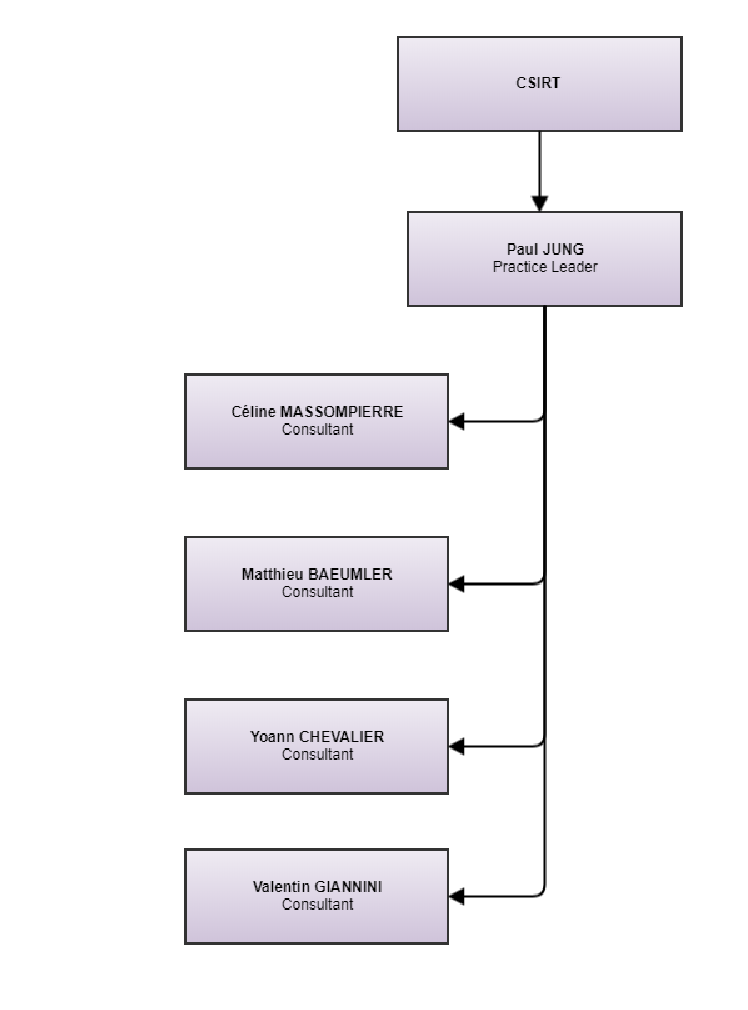
\includegraphics[scale=0.9]{figures/CSIRT_organigram}
  \caption{\gls{Excellium} \gls{CSIRT} organigram}
  \label{organigram}
  \end{center}
\end{figure}

\cleardoublepage

\chapter{Presentation of the project}
\section{Genesis of the project}
\subsection{Deception Technology: an emerging defense}
\blt{T}{he} term \textbf{Deception technology} might be unknown or obscure to you, and that is perfectly normal considering it refers to one of the latest trends in the cybersecurity field. Its concepts are however quite intuitive and easy to understand, and based on other well-known technologies such as Honeypots.
To put it simply, imagine you left something that will seem attractive in your enterprise network to any malicious actor, but booby-trapped in some way. Now hide it a little so only people that are tech-savvy and specifically looking for interesting or out-of-place data can find it. For example, a file with a name like \textit{DomainPasswords.xlsx}, containing erroneous credentials. Keep the persons on charge of the IT of this enterprise informed of the presence of this decoy. Then, just wait for somebody to trigger it. And voila! When the trap is activated, the probability of a false positive should be very low, and you most likely caught a person with malicious intentions.

The definition Gartner\cite{lib24}, one of the most famous advisory firms, gives of deception platforms is:\textit{[\ldots] centrally managed systems for organizations to create, distribute and manage an entire deceptive environment and its related architectural elements. These decoy workstations, servers, devices, applications, services, protocols, data elements or users are often virtualized, essentially indistinguishable from real assets and identities, and are used as lures to entice, engage and detect an attacker.}\eol Deception has been listed on the top ten of technologies for information in 2016 by Gartner\cite{lib17}\cite{lib16}. They suggested that before 2018, around 10\% of enterprises will use deception tools and tactics and \textit{By 2022, 25\% of all threat detection and response projects will include deception features and functionality, either embedded in their current vendor’s threat detection technology stack or through pure-play deception platforms, up from 5\% today}.

The main goal of the deception technology is to increase the Threat Detection and Response (\gls{TDR}) level of a company, by providing low rate of false positive, very accurate data and valuable telemetry. This approach is not the same as the modern cybersecurity that holds on big data analysis via \gls{SIEM} and data mining tools. Indeed, this technology favors a 'right data' approach rather than a 'big data' one. This is even more true for actors such as the \gls{Excellium} \gls{SOC}, which deals with hundreds of GB of logs every day. At this point, the need for more accurate and thus less numerous indicators becomes more understandable.\eol When a deception system is deployed inside an infrastructure, the blueteam gains the ability to hunt for anyone or anything interacting with deception items. It requires a time of setup and tuning in the beginning, to identify what are the legitimate interactions (for example a vulnerability scanner such as Qualys \ldots), and then you will see if there is a nasty agent which is already there scanning your network. But keep in mind that the deception technology is just another tool in the Defense in Depth (\gls{DiD}) approach, and should always be used in conjunction with classic cybersecurity technology. Indeed, deception is based on decoys, simulated services or fake documents. If an attacker manages to compromise the enterprise without interacting with any decoys, the only way to detect it is by traditional methods.\eol Deception technology also allows seeing if there is any suspicious activity inside your network.  

\subsection{Deception Technology: a detailed presentation}
\subsubsection{Deception Items}
Deception technology regroups all assets that can be considered as fake. We can identify these assets as follow: 
\begin{itemize}
    \item Fake servers also called honeypots,
    \item Fake data also called as honey-tokens,
    \item Data that lead to honeypots also called breadcrumbs.
\end{itemize}
Honeypots are servers seemingly part of infrastructure, but isolated and closely monitored. The literature also refers to honeypots as decoys. They can take several aspects. Their operating systems can vary, as the services shown to the attacker. These honeypots can provide either low or high interaction. A low interaction honeypot will just emulate legitimate services that a given server is expected to run, and only accept the most basic commands from the attacker. This makes the honeypot more secure, but it also reduces the information that can be gathered form the attackers. In the other hand, a high interaction honeypot will run the full-fledged service, recording all the attacker actions to give the security analysts detailed data on an ongoing attack. These high-interaction services can comes with a higher security risk and maintenance cost.

Honey-tokens are conspicuous data dropped in sensitive area of a network. One particularity is that they are stand-alone decoys, and requires little to no backend at all to work. That attackers, by exploiting these data, are tricked into sending information about themselves to the logs management system. These honey-tokens often take form of office or PDF files on network shares or workstations, with for example erroneous credentials for content, or crafted metadata that will make the office application generate a network connection to a monitored service.

The breadcrumbs are data deployed on real assets and that will lead an inquiring attacker to the honeypots. For example, simple DNS names hinting to high-value targets but whose records actually point to the honeypot. Or fake admin credentials or password hashes injected into the LSASS process, which when discovered and used by the attackers will generate an alert. These are called honey credentials. Connection shortcuts (\gls{RDP}) can also be used for the same purpose.



\subsubsection{Deploying deception technology}
The deployment process depends on what solution is chosen but we can summarize it with the most common methods.\eol The first part of the deployment is to gather information on the existing infrastructure, that means getting Proxy, \gls{DNS}, \gls{NTP}, \gls{SIEM} IP, company information, IP for honeypot, access for dropping honey-tokens. The network design of the company is also important in order to know where the deception should be put to be at the most relevant place.

The second part is to deploy all the deceptions tools, once all the company information has been gathered by the cybersecurity team. During the installation part, there is still need to have interaction with the network administrators of the company where the deception technology is being installed. For example, if you need some DNS records, AD accounts or anything else, you'll have to ask them.

Once the second part is over, you need to define the Use Cases for the company. Use cases define basically when the log deception manager has to raise an alert. This will define what the person in charge of managing these alerts will see when they arise, but also how to test the scenario, what have to done when there is a match, how to investigate the event and verify if it is a false positive, and how to escalate the incident when it appears to be a real threat.

Finally, the fourth part is the testing part where security analysts test the product in the client network infrastructure and whitelist all the legitimate users or engines that trigger the deception items.

\subsubsection{How does it work}
Once it is installed. The workflow will be divided in several parts: 
\begin{itemize}
    \item Installation of the deception item,
    \item An attacker managed to breach in the company network,
    \item The attacker triggers a deception tool,
    \item The analyst receives an alert,
    \item The analyst checks the alert and realizes it is an attacker,
    \item The attacker is discovered.
\end{itemize}
We can resume the deception work-flow with the figure ~\ref{deception_work}.
\begin{figure}[h!]
  \begin{center}
  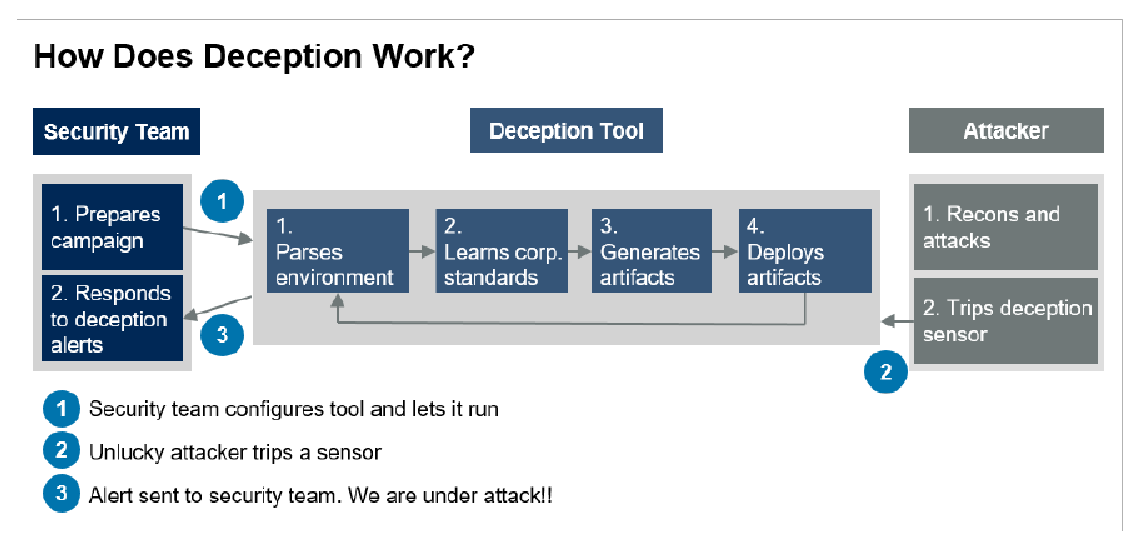
\includegraphics[scale=1]{figures/deception_works}
  \caption{How Does Deception Work? \cite{lib16}}
  \label{deception_work}
  \end{center}
\end{figure}

As we can see, the first action is to configure and install the deception system on the client network. Once it is done, the security analysts can just wait that someone triggers one artifact generated by the deception tool while doing their other day-to-day tasks. Once the artifact is triggered, the analysts follow what have been defined in the use case to determine if other actions are required.

\subsection{Deception Technology: the variable part in the deployment}
Every network infrastructure has its own particularity. Each company has its own way of writing documents, a specific log management policy and a different view on what have to be considered as critical for its business. That's why deception technology cannot be set up twice the same way. For example, the naming policy is very fluctuating, as the IP attribution is. One advantage of the deception technology is the ability to look like a real asset. That why a preparation phase has to be done prior to any deployment.

\subsection{Deception Technology: pro and con}


Let's do the pro and con for deception technology.The main advantage of deception technology is that the false positive rate of deception is low. Indeed, by the design of how deception works, the simple connection to one deception item is not supposed to happen.\\
Another advantage is that it enables to a security engineer to use his knowledge of his infrastructure for its own defense.\\
However, deception also has drawbacks. For example, this is not something that will be triggered all the time. An attack could be successful and undetected if the attacker does not trigger deception tokens. Moreover, some tools that detect some kind of deception are already available  so a pentester aware could dodge some traps. Furthermore, what it is complicated in deception is that testing is quite complicated because attacks are always new.

\section{Goal of the project}
The main goal of this project is to be able to produce a working Proof of Concept (\gls{POC}) of deception technologies. A definite plus for this project would be to deploy this \gls{POC} on client infrastructures without a lot of effort for the person who will be in charge of the solution installation.

The beginning of the project will be to get familiar with all information dealing with deception technology. That means reading the available literature and documentation about deception, but also broadening this with related topics such as how to make a deception network safe. The result of this first step is a state of the art document to be uploaded on the \gls{Excellium} Confluence. The main parts of the state of the art document are:

\begin{itemize}
    \item Deception System,
    \item Open Source Honeypot,
    \item Open Source Deception Tools,
    \item \gls{IPS}/\gls{IDS} Open Source.
\end{itemize}

The second part of the project is to establish the design of the application. In a simple way, this objective was to draw the design solution at a network level and software level (see part  \ref{design}). This gives the solution a body and help to imagine how will the final product will look like, helping to think about the entire solution before even doing it.

The third part consists in building the solution on what we worked before. This took place on the virtualized environment of \gls{Excellium} (VMware ESXi) in order to see if the solution is something that we are capable of doing. It also helps to face the potential problems that someone could encounter during a client installation, but in this case it is easier because we have 'master' over the network.

The last part is to install the solution that have been tried at \gls{Excellium} in a client infrastructure. This part is the part where the project is truly evaluated. 

\section{Final deliverable}
The final deliverable has to be as simple as possible. It will be divided in several parts. The first big part will be a documentation one. In this part will be presented the state of the Art described previously, but also the design solution (network and application). It will also contain all the documentation on how the solution is working, and how someone can install it in a client infrastructure. Another deliverable is the templates of the virtual workstations that was produced during the solution elaboration.

The documentation part is available in the \gls{Excellium} Confluence under the section:  Computer Security Incident Response Team Home - \gls{CSIRT} TRAININGS - Internal deception device.
The templates are available on the ESXi in the trainee folder.

\chapter{State of the Art}
\blt{T}{his} project regrouped a lot of different technologies. I had to increase my knowledge, or learn, about network infrastructure, network protocols, pentester attack plans and of course all that was a part of my internee subject. That is why the main parts of my state of the art are: 
\begin{itemize}
    \item Deception System,
    \item Deception Tools,
    \item Network Security Tool,
    \item Orchestration,
    \item Kill chain.
\end{itemize}
Another version of this state of the art was made with Microsoft Word in the beginning of my internship and is a little shorter.

\section{Deception System}
Here is the part where I'll be talking about the most relevant technologies in place within the deception system.
The amount of information on each product differs because most deception systems are black boxes, and the information that I gathered are only the results of the information found on Internet. 
Deception Systems are cybersecurity systems that are incorporated in a company network to fool potential attackers. What makes them useful is that there are very accurate, and easy to deploy.
Every deception System works approximately the same way: first, they scan the network looking for some patterns in the network (they often use machine learning), after that, they spread their endpoints and deception items over the networks.

I have done my state of the art of deception on the products presented in the table \ref{tab:search}

\begin{table}
	\centering
	\begin{tabular}{|c|c|}
		\hline
		\textbf{Vendor}  & \textbf{Name of the Solution}                  
		\\
		\hline
		Acalvio            & Shadowplex\cite{lib4}
		\\
		\hline
		Attivo             & ThreatDefend Platform\cite{lib2}
		\\
		\hline
		CounterCraft       & Cyber Deception Platform\cite{lib}
		\\
		\hline
		Cymmetria          & MazeRunner\cite{lib5}
		\\
		\hline
		Deceptive Bytes    & Active Endpoint Cyber Defense
		\\
		\hline
		Fidelis Security              & Fidelis Security Deception                                                            
		\\
		\hline
		Illusive Networks  & Deception Management System                              
		\\
		\hline
		PacketViper        & PacketViper                             
		\\
		\hline
		Smokescreen        & IllusionBLACK                               
		\\
		\hline
		TrapX              & DeceptionGrid                              
		\\
		\hline
	\end{tabular}
	\caption{List of Deception Systems}
	\label{tab:search}
\end{table} 
 
\subsection{General offer}
The general offer is what is classic to see in deception system. All of them provide main installation via virtualisation.
Deception systems are based on five main pillars: Manageability, Discoverability, Undectability, Interoperability and Cost-effectiveness. They all provide all of decoy. They often works with a first network scan for knowing what they have to do and continue doing it continuously for having a constant knowing of network state. This allows having an automated deployment and an optimal deployment.\\
All these systems are managed by a platform that allows the client to follow time to time what alerts are triggered and what action have to be taken. 



\subsection{Specific offer}
Every system doesn't provide exactly the same kind of deception service. Here we are going to see what are the main differences.
Every system uses virtualisation, but the hypervisor used is not the same, some use KVM, a linux open-source hypervisor (cymmetria for example) and some the vmware hypervisor: ESX.\\
Some provide API for easier implementation.\\
Some other offer cloud tokens for the three main cloud platform:  AWS (Amazon cloud), Google cloud and Azure (Microsoft cloud).\\
CounterCraft offer a unique deception which is called wifi deception and use a physical item to fake a wifi endpoint.
Finaly, the more advence system provide active response. That means that these solutions enable security teams to scripts and automate workflows for active response and investigation (Fidelis Security Deception for example).



\subsection{Exploitation Model}
There are two kinds of exploitation model presented in all the deception system that I have study.\\
The first one is the model that is told as DaaS (Deception as a Service). This model is an installation that use the example of the cloud. Service and software are based on distant server.\\
The other model is the classical model where all the solution is installed on the client infrastructure.\\
The first one is instresting because the client doesn't have a lot to take care off. The provider of the solution deal with the management of what is installed. But the second one is more intresting regarding security issues. Indeed with the solution in intern, the security is handle by the client and the client only have to trust its own infrastructure.  


\subsection{Pricing}
There is two kinds of pricing in the field of deception system. A global pricing which turns between twenty thousand dollars (Acalvio) and fivety hundred dollars. And a pricing by sensor which is around five hundred and one thousand dollars by sensor. The last payment offer is by user, for example Guardicore offers its solution for 60 dollars by user.

\section{Deception Tools}

\subsection{Deploy-Deception \cite{lib20}}
Deploy-Deception is a powershell module that is able create active directory decoy objects. This module has to be run on a Domain Controller with a domain admin account. This decoys are based on domain object flags and attributes. For example the flag 'PasswordNeverExpires' is a flag that interest attacker because this password could be very old and often easy to crack. 
There are five different kind of active directory objects that can be deployed: 
\begin{itemize}
    \item UserDeception: that creates a user account with some attractive property and flags and monitor any access in read to its property,
    \item SlaveDeception: that creates a slave and a master which have 'GenericAll' right over the slave: any interaction to the master or the slave is monitored,
    \item PrivilegedUserDeception: All is in the name, that create a privileged user, often member of the domain admin group but on which nobody can log on. Any interaction with this user is monitored,
    \item ComputerDeception: that create a computer object with 'Unconstrained Delegation' property enable. This is an interesting property for having Ticket Granting Tickets, a ticket which allow you to access to some services. Any interaction with this computer object is monitored.
    \item GroupDeception: that create a group which is member of the dnsadmin group. Any interaction with this group object is monitored.
\end{itemize}
Any monitor action is done via the event viewer. The principal events that are monitored are: 
\begin{itemize}
    \item the 4662: 'An operation was performed on an object',
    \item the 4768: 'A Kerberos authentication ticket (TGT) was requested'.
\end{itemize}
Those events are triggered when the objects are accessed or requested. It could be interesting, but the inconvenient is that it is mandatory to be domain admin to run that, and that in a client infrastructure, it is hard to have this kind of access.\eol All the code is available in Github and totally free.

\subsection{Canary Token \cite{lib9}}
\subsubsection{What is it ?}
Created by Thinkst, this technology is based on a tool that can create files called deceptions tokens or honey tokens, that are triggered during the token opening. These tokens are often linked to a webserver that is contacted every time a honey token is triggered. What is called token could be different kind of files like URL, DNS, email, word, PDF, windows Folder, dll, exe, docx…

A basic user has access to a website: \textbf{\textit{https://canarytokens.org/generate}}. This website ask the user to give:
\begin{itemize}
    \item The kind of canary token that he wants,
    \item A webhook url or an email address; this is where the alerts will be sent,
    \item A reminder note to send when the canary token is triggered.
\end{itemize}
Once these information are given, the user download a web-generated file that correspond to the kind of file that the user specified before. The user will drop this file in a place that need to be monitored. And finally, when the token will be triggered, the user will be notified either by mail or by the webhook URL.
The interface looks like the figure \ref{fig:canary}.

\begin{figure}[h!]
  \begin{center}
  \includegraphics[scale=0.7]{figures/Canary}
  \caption{Canary Token Web Interface \cite{lib22}}
  \label{fig:canary}
  \end{center}
\end{figure}


For a company, Thinkst provide a github where there are python scripts and a docker image that allow a quick installation of the token generator website. It provides also more advance information when one canary token is triggered. 


The most relevant are PDF, docx and URL. These tokens only are triggered when they are open by classical applications, for example if an html is created with a URL pointing to the server is opened by a cat command, the token will not be triggered.

\subsubsection{Pros and Cons}
The pros for this solution is that can be easily spread on the network, this is not something heavy to drop on the network and when canary tokens are triggered we can choose by what means the alert can be sent. Furthermore, the kind of notification we receive is quite complete : there are information about the IP which triggered the document, the note that have been writing down when the creation of the token mentioned, and finally there is the timestamp.
The cons for this solution is that we need at least one server to create the canary tokens. Moreover, some tokens need permissions to be triggered (pdf, docx …).



\subsection{Domain Controller Enticing Password Tripwire (DCEPT)\cite{lib10} \cite{lib11}}
This tool is based on the pass-the-hash attack which consist on extracting hashes credential stored when an LM or NTLM authentication have be done. The DCEPT agent inserts fake data on the cache in order to deceive the attacker once he is a local admin on the endpoint where the DCEPT agent is installed.  

This is a tool that works with three endpoints:
\begin{itemize}
    \item One agent written on C\# which caches honey tokens,
    \item One server that generate, issues and manage the honey tokens,
    \item One component that listen logon attempts.
\end{itemize}

The pros for this solution is that it is a very tricky one and that the code available. But the cons it is that the solution use many resources, that the solution has a bad detection ratio (pentester get there late, they rather find creds first), and this solution needs to use nonAD credentials (for detection, because there is no sniffer).

\section{HoneyPot}
One of my main interest was about HoneyPot, the central point of my subject. I found a great GitHub \cite{lib11} that listed nearly all the most interesting links to open-source honeypots and deception tools.


Before presenting the most interesting honeypot that I found, I will present the principals characteristics that define a honeypot.
The term honeypot first refers to the pot containing the sweet product that bears love unconditionally. But it also refers to the cybersecurity assets that are set to fool attacker by simulating real IT assets.
One of the question that you have to ask yourself when you first install a honeypot is how well it is secured. An attacker must be flagged when he contacts an honeypot but he also must not be able to gain real access of the honey otherwise he could do more damage, especially if this is a honeypot integrated to a real production environment.
According to that, two categories of honeypot can be defined, the high level interaction honeypots and the medium level interaction honeypots. The level of interaction is based on what an attacker is able to do on the honeypot. While a high level honeypot is interesting to study the kind of attack a hacker can do, and is therefore more valuable for cyber research purposes, a low interaction level is more interesting for generating alert and making a company aware that someone is probably targeting it. We will focus our analysis on the last category because it corresponds to the kind of honeypot I was looking for. 

I present in the figure \ref{fig:hp} the most interesting honeypots that I found. There is a lot of available open-source honeypot on github or other platforms. Some choice have to be made. The CSIRT is used to use python so I choose to focus mainly on the technologies that use python (Python 3 is better, but there are still a lot of project in 2.7). One other thing very interesting is to see what services are monitored. SSH, HTTP/HTTPS and data base are the three main services emulated because there are frequently under attack and often exposed. Moreover, what was put on the figure \ref{fig:hp} is the years of the last commit on the project. Indeed, a project that have a recent commit shows that it have a community behind and that it is maintained. This is a good thing because protocols can evolve and it is good to have a product that evolve at the same speed. Finaly, OS on where honeypots could run are also important because if the honeypot run on licensed OS, that should be taken into account so as the OS company park.

\begin{figure}[h!]
  \begin{center}
  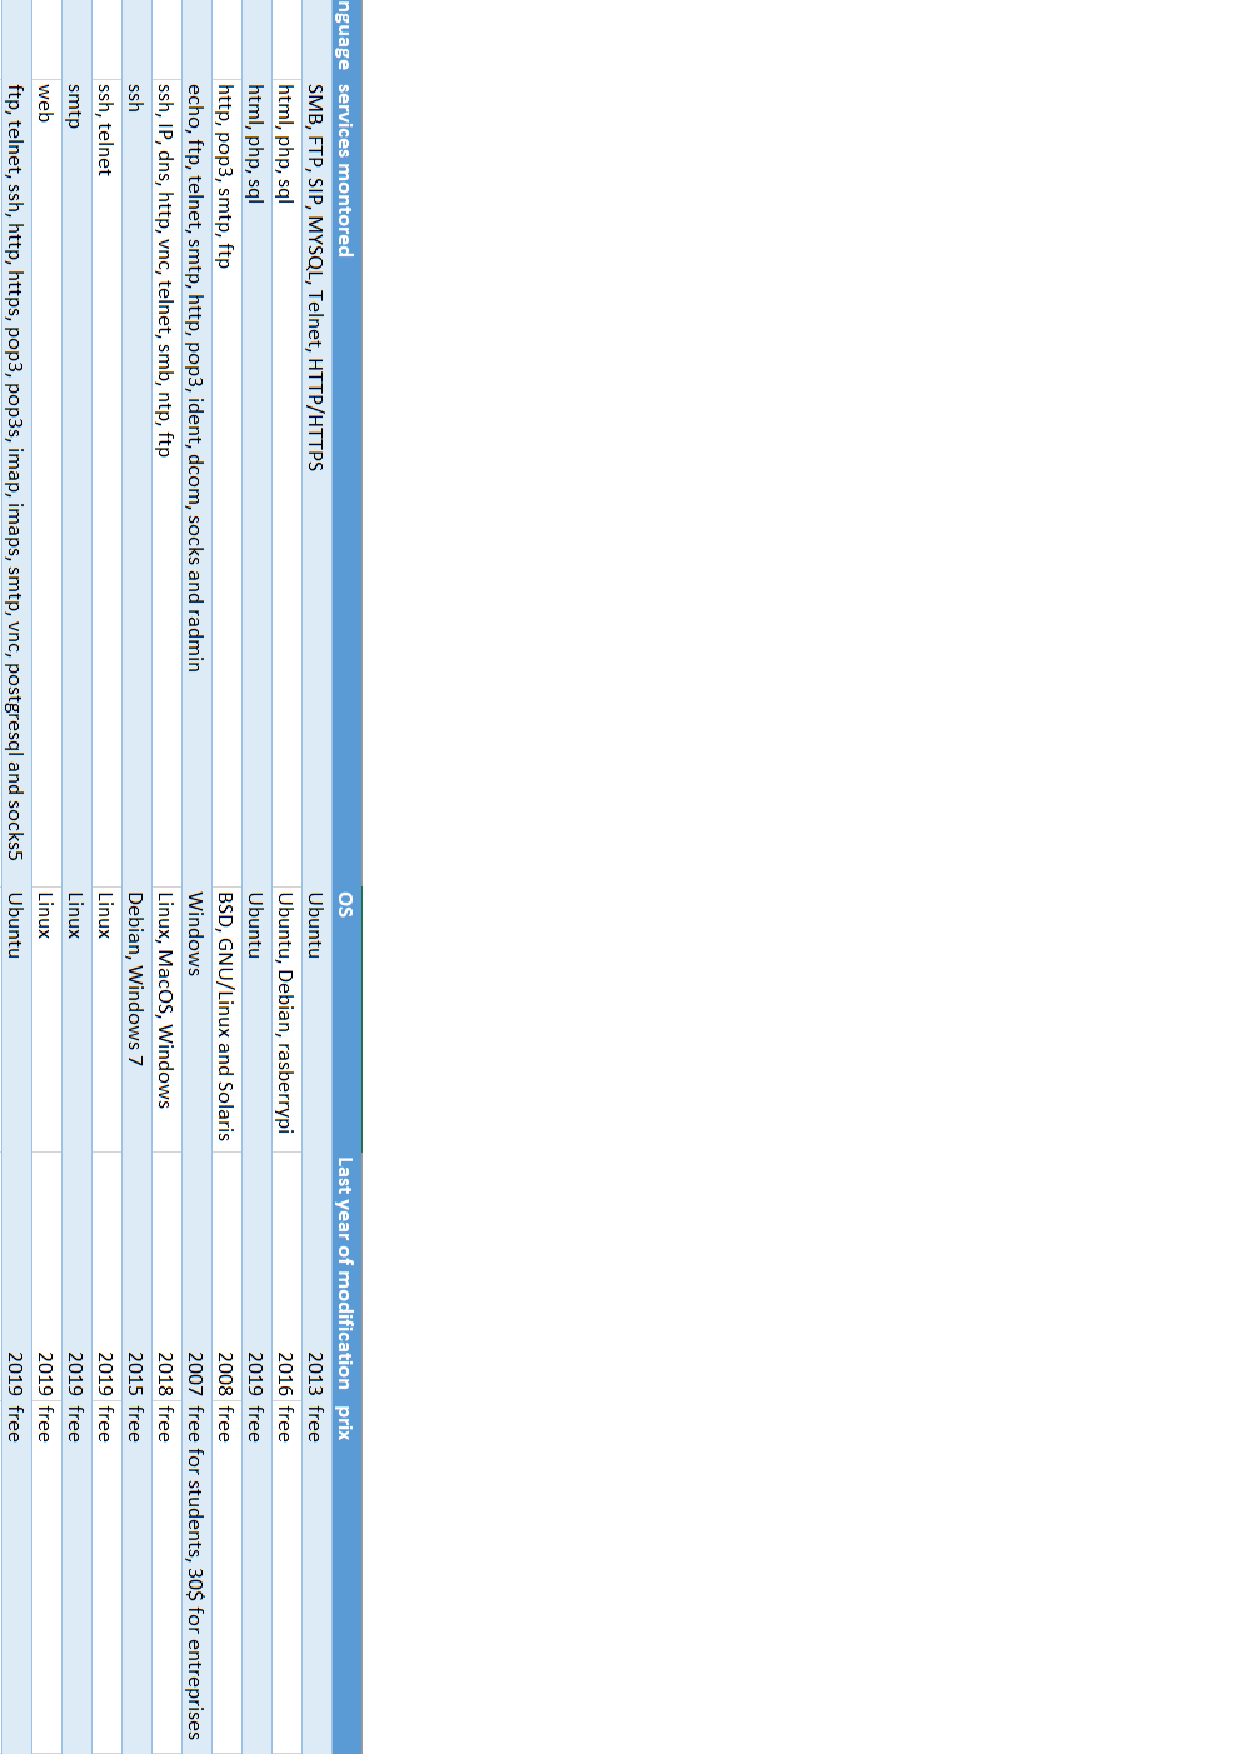
\includegraphics[scale=0.7]{figures/honeypot.png}
  \caption{State of the art honeypots}
  \label{fig:hp}
  \end{center}
\end{figure}

\section{Network Security Tool}
As mentioned earlier, the security of the environment is at stake each time a new equipment is deployed. In order to ensure a high level of protection, I've done a comparative study on the \gls{IPS}/\gls{IDS}  (Intrusion Prevention/Detection System) technology. The two main targets of my state of the art was Suricata and snort. The choose of the study of the two of them was done because they are both free, open-source and well documented. I also study the functioning of iptables for natting purpose.

\subsection{Snort}
Snort is a free open-source networks base \gls{IPS}/\gls{IDS}. Available since 1998, this is a tool that have a big group of user. He is using a wildely known language, the C. One good point of this tool is its scalability and its flexibility. Indeed, it can be deployed in multiple network environment and on several OS. Snort is rule-based \gls{IPS}/\gls{IDS}. That means that Snort will log / block only the traffic that is told by the rules to be logged / blocked. When you are using Snort, four choose are open for having rules: 
\begin{itemize}
    \item Using the basic rule set providing by snort,
    \item Using rules shared by the snort community,
    \item Using rules that you bought, for example Talos ones,
    \item Creating your own rules.
\end{itemize}
The ruling syntax of snort is quite basic, you can see an example of one in the picture \ref{snort}. You can define the ports, the ip addresses and the protocols to monitor. This way, the rule defined on figure \ref{snort} will make an alert saying "ICMP Attempt Attack" whenever an ICMP packet which have a source ip address 192.168.1.10. 
\begin{figure}[h!]
  \begin{center}
  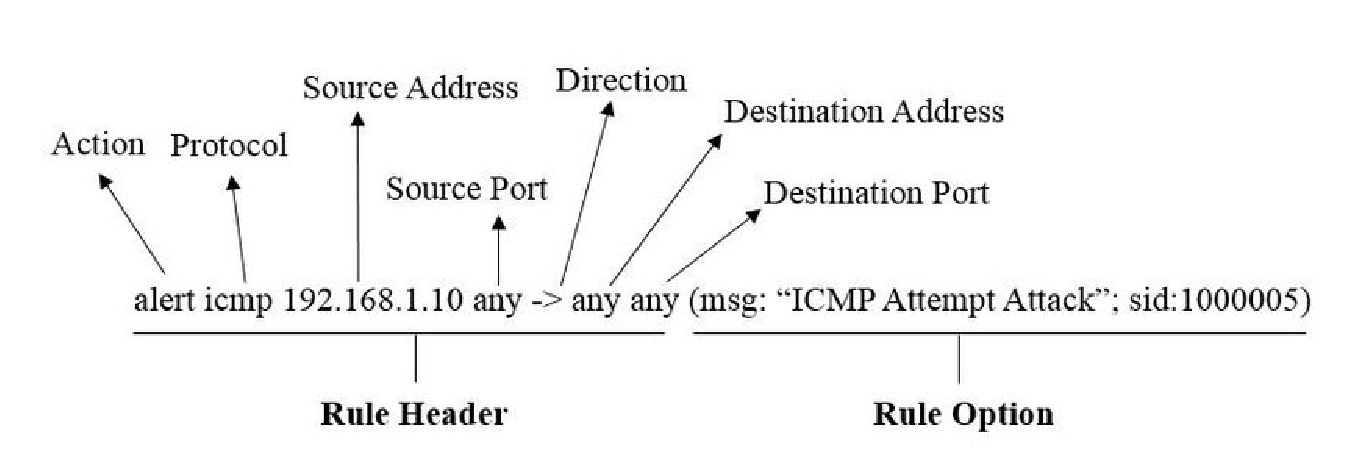
\includegraphics[scale=0.7]{figures/snort_rules}
  \caption{Snort rule \cite{lib22}}
  \label{snort_rules}
  \end{center}
\end{figure}

The main drawback of Snort is that this is not a solution "application aware". That means that snort is not able to detect a traffic HTTP, it could only detect a TCP traffic on port 80 for example. 
A notable and famous thing about snort is his big pig as a logo.

\subsection{Suricata}
Suricata is also a free open-source networks base \gls{IPS}/\gls{IDS}. Its first version came out in 2009 and was developed by the Open Information Security Foundation (OISF). The use of Suricata and Snort is  quite the same. Indeed Suricata is also rule-based. He also has its own ruling language but also support most of the rules written for snort (the Talos rules works).
The rules query are like presented in the figure \ref{suricata}.

\begin{figure}[h!]
  \begin{center}
  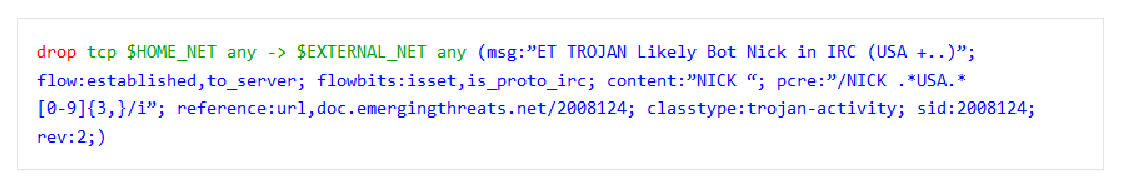
\includegraphics[scale=1]{figures/regles_suricata}
  \caption{Suricata Rules}
  \label{suricata}
  \end{center}
\end{figure}
In the example figure \ref{suricata}, red is the action, green is the header and blue are the options. It is really close to snort language.\eol The main advantage of Suricata over Snort is that Suricata is younger. Thus, Suricata functionality widely used nowadays like multithreading and application detection. 


\subsection{Iptables}
Iptables is free software embedded with Linux kernel. The purpose of iptables is to manage packet and it is mainly used to manage and configure the Linux kernel firewall. Iptables has been developed in the C language and is a part of the Netfilter framework. Iptables is used in command line. These commands are tables-based. There are four tables: 
\begin{itemize}
    \item Nat table: used for address translation,
    \item Filter: used for packet filtering,
    \item Raw: used for configuring exemptions from connection,
    \item Mangle: used for special purpose.
\end{itemize}
A table is a set of rules divided into chains. According to routing decision, every couple table-chain crossed will have his rules triggered. This process can be illustrated by the picture \ref{iptables}. In the figure \ref{iptables} the first routing decision is to determine if the packet has to destination the endpoint where iptables is installed or if the packet has been forwarded. According to this, different rules will be triggered following the path of the figure \ref{iptables}.

\begin{figure}[h!]
  \begin{center}
  \includegraphics[scale=0.4]{figures/ip_tables}
  \caption{Iptables workflow \cite{lib21}}
  \label{iptables}
  \end{center}
\end{figure}

The rules are organized in list, and the rules are executed in order. For example if there is a rule that drop all packet from an ip X and an other rule that accept all packet from an IP address X is set, the one that will define the becoming of the packet will be the one on the top of the list.

A classical iptables query is: 
\begin{center}\lstinline|sudo iptables -A  -i <interface> -p <protocol (tcp/udp) > -s <source> --dport <port no.>  -j <target>|\end{center}
For adding rules in iptables the user should have by default root rights. The -A option mean adding the rule in the last position of rule set. The other option i, p, s and dport specify the targeted packet, other property can be selected as sport for example. The j option specify what to do if the options match, for example the target LOGGING will send the packet to the kernel log. Thus, thus rules will send to the target -j  the packet coming to -i on port --dport with the proctocole -p coming from -s.
\eol Iptables is a very usefull tool on ubuntu because it is available from scratch and have a lot of tutorials online.

\subsubsection{Saving rules}
The working process of Iptables is to destroy all rules after each reboot. As a workaround, a solution is to install the package 'iptables-persistent'. 

\section{Orchestration}
Thomas Erl define the orchestration as \textit{[\ldots] the automated configuration, coordination, and management of computer systems and software} \cite{lib19}. For maintaining my network infrastructure, the subject of the orchestration was something to think about. I had several chose to make between the ease and the practical. I'll show you the three options that I though for this part.
\subsection{Puppet}
Puppet an open-core software configuration management tool. It permits to deploy new configuration through easily. It is based on a client-server architecture. The server is called master, the workstations are called slaves. The slaves often communicate with their master and ask if there is a new configuration to apply. When there is one the server managed to give the slaves their new configuration. It is then easy to deploy a new update just by pushing something to the master, which will be, after, in charge of pushing it back to the slave concerned.
The advantage is the capability of a quick and centralized deployment of configuration. But the drawback is that a server is needed to install the puppet master and the slave also have to be configured.
\subsection{Debian Package}
Debian package is well known and used by developers. Debian packages integrate very well into the entire system.
One advantage is that thanks to the fame of the packaging, there are a lot 

The packaging work flow is usually like this:

\begin{itemize}
    \item Step 1: Rename the upstream tarball,
    \item Step 2: Unpack the upstream tarball,
    \item Step 3: Add the Debian packaging files,
    \item Step 4: Build the package,
    \item Step 5: Install the package. 
\end{itemize}

This is a good way of installing and deploying a craft package because it doesn't need that much user interaction and user are used to use it.

\subsection{Bash script}
A bash script is the simplest way of installing and configuring a software. The advantage is that an advanced user can see what is really happening, and that this is quite simple to do.
A bash script is a script beginning by \#!/bin/sh, it is basically a plain text that are composed by many commands.

\section{Kill Chain}
The Cyber kill chain in cybersecurity, originally developed by Lockheed Martin\cite{lib25}, comes from the military kill chain which consists of an end-to-end process. In cybersecurity, this term designates all the steps followed by the attackers to finally achieve the goal of his mission. This often means be administrator of the domain. This chain is divided into seven main parts that are: 
\begin{itemize}
    \item Reconnaissance,
    \item Weaponization,
    \item Delivery,
    \item Exploitation,
    \item Installation,
    \item Command and Control,
    \item Actions on Objective.
\end{itemize}

This is a framework well known in the cybersecurity industry that everybody in this field should be aware of, because when you build a cybersecurity tool, you have to know in which part of the chain will you potentially catch the attacker.\eol The kill chain can be represented by the figure ~\ref{killchain}.

\begin{figure}[h!]
  \begin{center}
  \includegraphics[scale=0.5]{figures/Kill_Chain}
  \caption{Kill Chain \cite{lib18}}
  \label{killchain}
  \end{center}
\end{figure}

This figure~\ref{killchain} is a representation of all the possible steps that are done by an attacker and where each part can go into a part presented above.

\subsection{Reconnaissance}
The reconnaissance part is the part when the attackers regroup information about the target. They will gather information that you can have easily or not. For example they will take the public IP available via DNS records, or look for open port and IP potentially vulnerable via scanner like Shodan\cite{lib26}. They will also gather company information, such as the basic email pattern : 'firstname.lastname@company.com' for example.\eol In this part there is nothing we can't do with actual deception. We could try to spread fake information through internet but this could have a bad impact on the society and this is therefore not advised. 

\subsection{Weaponization}
The weaponization part is when the attackers prepare something that will allow them to have a first foothold in the company. What is most frequent is either a malware that will be dropped on a company, a phishing website that is customized for the company targeted, a leak of passwords collected on the darknet \ldots
In this part, there is also nothing that we can do, at a deception level.

\subsection{Delivery}
The delivery part is the part when the attackers deliver the 'weapon' that they collected during the previous part. If the weapon is a malware, the delivering process could be sending a mail to the victim with the malware embedded as an attachment. In this part, there is also nothing that we can do, at a deception level.

\subsection{Exploitation}
The exploitation part is the part when the attackers have dropped their payload and it has been activated. For example, if a malware has been downloaded as an executable file and that the targeted victim execute it. Here, a deception tools could be triggered. For example, there is the worm malware category that regroups malware using software vulnerability to spread over the network. If this malware tries to spread, we could know.

\subsection{Installation}
The installation part is the part when you install the malware backdoor on the victim asset. This part is not a part of all attacks but it occurs more often than not. A backdoor is a remote access that gives a persistent access for the attacker. This could be seen if the attacker tries to do it on a deception asset.

\subsection{Command and Control}
The Command and Control (\gls{C2} or C\&C) part are the part when the attackers make an easy access to the targeted network from a server. The name of the subsection comes from the name that are given to these kinds of servers.

\subsection{Actions on Objective}
The action on objective part is the part when the attackers have the access and the ability to do what for they came for. That means steal juicy data, compromising a service / network, spying\ldots Here deception is also very interesting. A text file \textit{'domainpassword.txt'} in an admin folder of a shared file could be very attractive to an attacker.

\cleardoublepage

\chapter{Design of the solution}\label{design}
\blt{S}{ome} people like to just jump into developing without writing down and without thinking about the project in a global form. That's not what I have done. I chose to take time to think about the global design of my future project. Indeed it is better to think about modularity, maintainability, performance, usability, traceability and deployment before the beginning of the project than think about it at the end.

\section{Network Configuration}
The application will be deployed via the ESXi. The ESXi deploys three workstations: two Ubuntu and one Windows workstation.

The choice of the ESXi was made because, first, it is easy to deploy workstations of any OS that already has anything needed pre-installed on them. This is done via the help of VMware templates. The choice of ESXi was also done because of monitoring information that are provided via the vSphere interface.

The first Windows workstation will be created with an attractive AD user name, a RDP emulation and a folder shared with anyone (configuration bait). It will only need one IP address and a DNS record.

The first Ubuntu server emulates \textbf{n} (number to define) services and have \textbf{n} IP addresses, one for each service. The number of IPs could be less than \textbf{n} because it is not surprising for an IPs to have several services that are running.

The second Ubuntu server is there to act as a listener and filtering network flow between the outside (client's network) and the VMs decoys. This Ubuntu server is also charged to detect and stop targeted malicious activities on the other VMs with the help of an \gls{IDS}. It will NAT all the traffic which has for destination the decoys.

Some fake data will be uploaded on the Share Server of the company and the opening of those documents will trigger alerts to the first Ubuntu server. This functionality will only be possible if the customer allows us to drop fake data on sensitive network emplacement. If the customer want this functionality, the fake documents will be dropped on a shared ftp server for example.

The log report will be done via the \gls{SIEM} which already has a route to the \gls{SOC} of \gls{Excellium} Services. All the logs will be sent to the \gls{SIEM} via the second Ubuntu server. This way all the traffic coming and leaving from the decoys will pass through the \gls{IDS}. This is done to have the best security flow. 

The access to the ESXi for the installation and for the admin processes is done via the route already configured for the \gls{SIEM} installation and monitoring. If there is no route, one need to be configured between \gls{Excellium} and the customers.\eol Access to the Internet will be granted by the link between the ESXi and \gls{Excellium} (or if possible, by the Internal Company Proxy).

The schema of this architecture can be seen in the figure \ref{fig:network}. This is a layer 3 architecture and so we don't see the layer 2 architecture. But the architecture of the decoys will be divided in two separated VLANs. An administration one where only administrators will have access, and a more open one.

\begin{figure}[h!]
  \begin{center}
  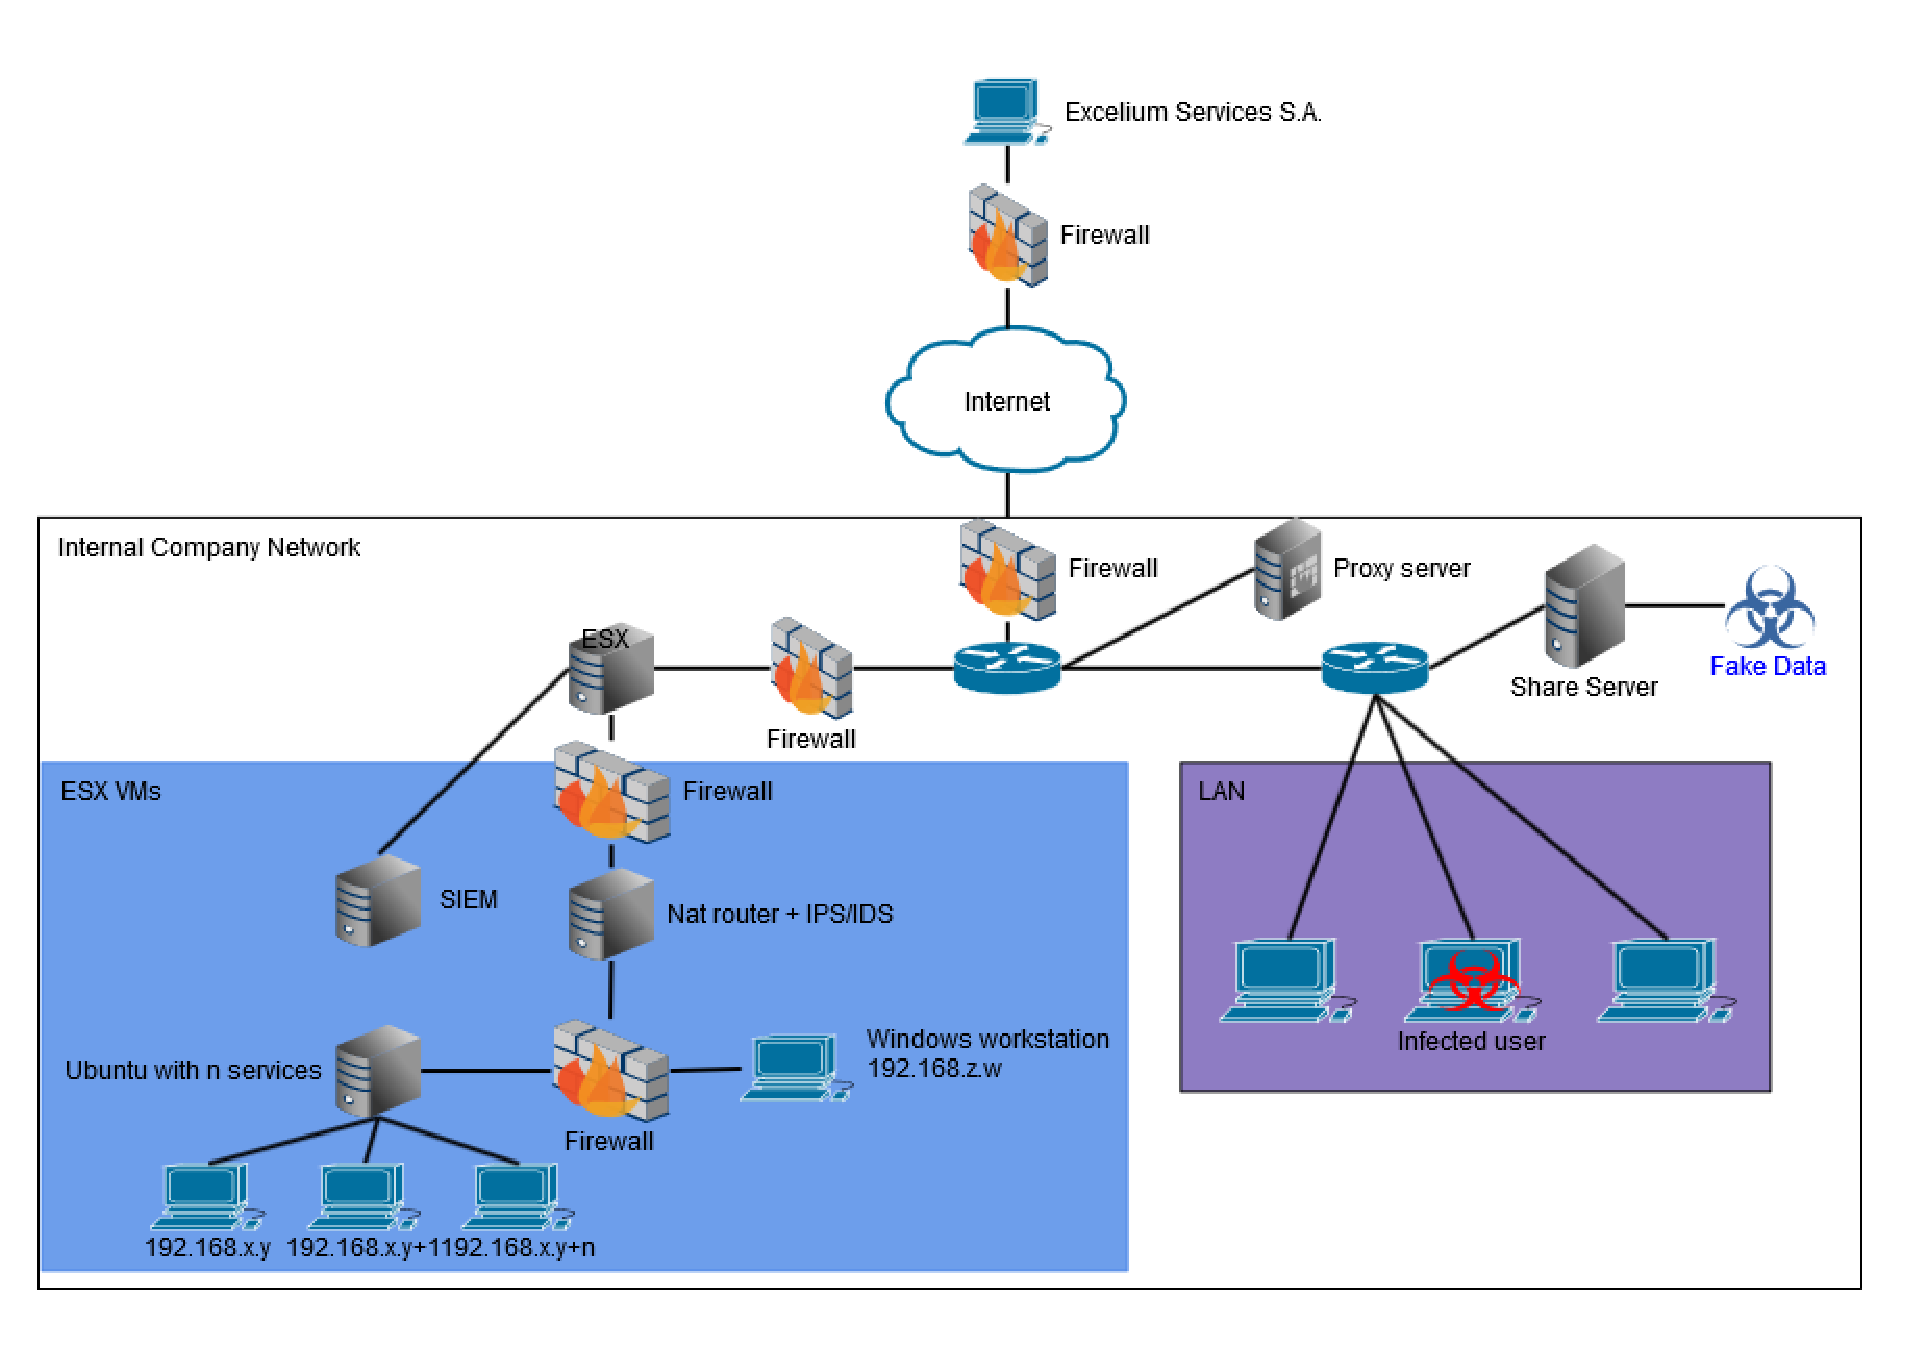
\includegraphics[width=\linewidth]{figures/network}
  \caption{Design of the deception network}
  \label{fig:network}
  \end{center}
\end{figure}



\section{Application selected}
In this part, we will discuss the software and the OS that we deploy on the three VM's that we install on the customer ESXi.


As it can be seen in the diagram below, we use several apps.
First of all we use Python 3 which is the main scripting language that we use for this application. With the help of python 3 we use Pysyslog and Heralding which are python 3 packages. The choice of Heralding was done by the need of the \gls{CSIRT} to have a global scripting language: python 3. Moreover, Heralding is a very good honeypot that is easy to download and run. It provides good logging information, and this is really important for helping \gls{SOC} engineers to determine if received alerts are real positive.\eol The Ubuntu honeypot will also have a webhook server which is linked with decoy data installed on the share Server. Once these fake data will be triggered, the webhook will collect information and forward them back to the \gls{SIEM}. The webhook selected is the one provided with the package webhook of ubuntu. The choice was made based on the ease of installing.

We use Cacti, an open-source web based network monitoring tool on the Ubuntu controller machine to prevent our application from saturating the network and specially not to overflow the bandwidth. The web based application needs a server web to work, that's why we also use Apache on this server.

We use Suricata (an \gls{IDS}/\gls{IPS} open-source) to forbid malicious activities on our VMs. The choice of Suricata over Snort was made because of the experience I had on the two \gls{IDS}, on the performance on the two solutions and on the ruleset available. Moreover, Suricata logs are already parsed by Excellium \gls{SOC}, so it will be easy to parse logs of the clients \gls{SIEM}.

Sysmon was also something that was installed on the Windows workstation. Sysmon is a Windows service that is useful in cyberhunting because it brings more detailed logs about system activity. For example, network connection, process creation are well logged with Sysmon. 

For the logging part, the module rsyslog was chosen. It appear to be a logic chose because this is the one that is provided with the installation of ubuntu. It is also one that have a lot of documentation online and my tutor knew the most.

A recap of all application used is done in the figure \ref{fig:app}.
\begin{figure}[h!]
  \begin{center}
  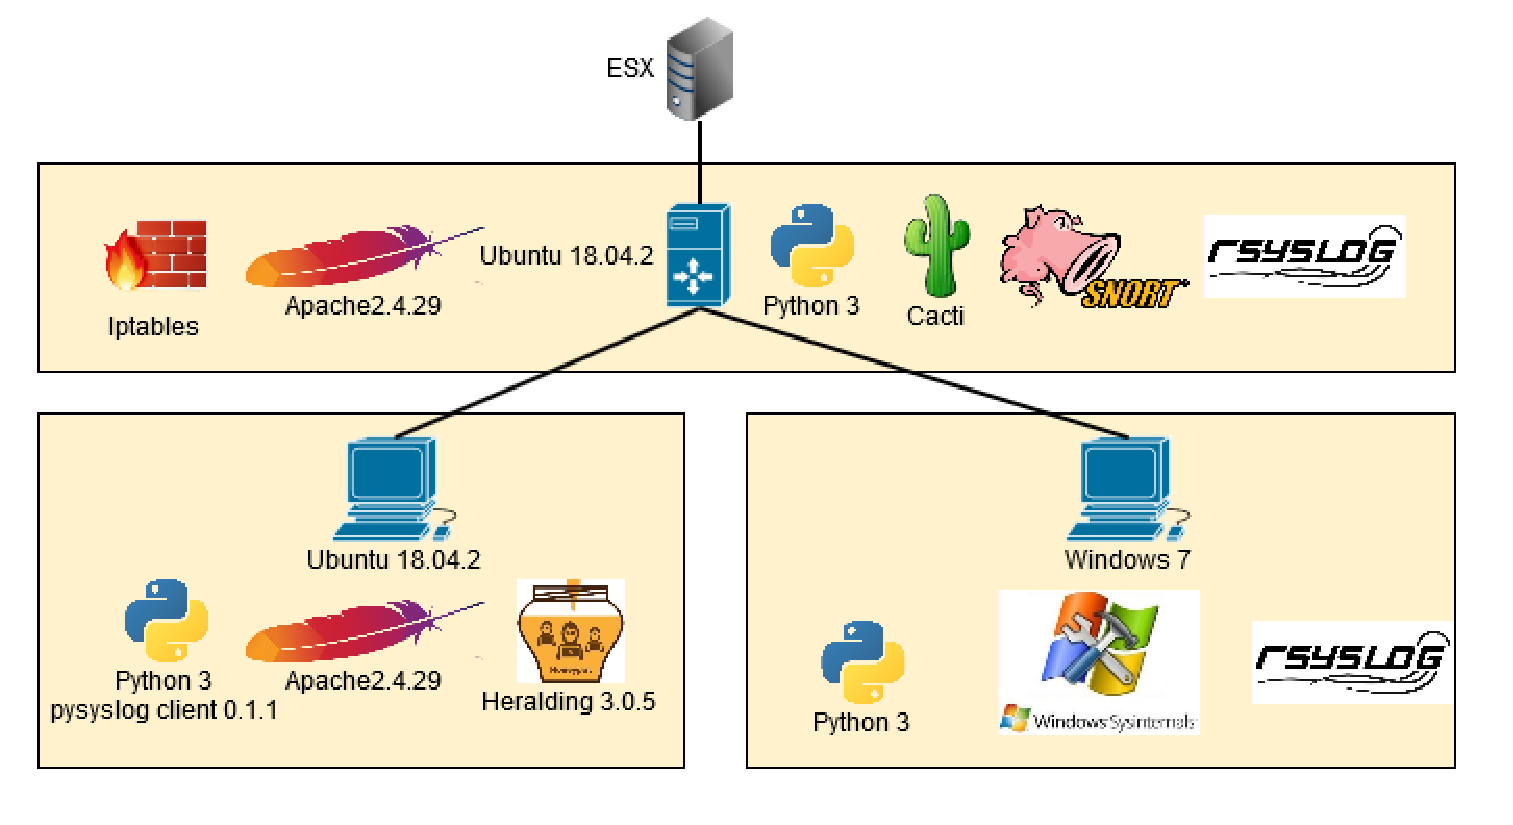
\includegraphics[width=\linewidth]{figures/application}
  \caption{Design of the deception applications}
  \label{fig:app}
  \end{center}
\end{figure}

\chapter{\gls{UAT} deployment}
User Acceptance Testing consists of a process that verify if a solution works for the final user. Thus, the environment need to match as close as possible the final environment where the final solution will be implemented. The use case of the solution should also be relevant to simulate a real utilization.
A good (\gls{UAT}) deployment can give a first look to the client and make him see what the product looks like.
(\gls{UAT})
\section{\gls{UAT} environment}
\blt{T}{he} \gls{UAT} environment for \gls{Excellium} is his own ESX platform. ESX stands for the VMware ESXi product which is an enterprise-class, type-1 hypervisor developed by VMware for deploying and serving virtual computers.\eol Virtualization has a lot of advantage. For the project, it will help by deploying easily the deception infrastructure. Indeed, in some click, an ESX administrator can deploy an OS on the network via the graphic web interface: vSphere. This interface is helpful because it allows you to have a quick look on the VM. \ref{fig:esx}

\begin{figure}[h!]
  \begin{center}
  \includegraphics[width=\linewidth]{figures/esx}
  \caption{vSphere interface}
  \label{fig:esx}
  \end{center}
\end{figure}


The interface of vSphere also allow to have a quick look of the physical element of the vm. On the figure \ref{fig:esx}, on the right, there are the cpu, memory and storage usage value that are shown. This allow a quick monitoring on the VM.


Templating is also available in ESX. By simply converting a virtual machine into a template you can whenever you want to deploy the exact same virtual machine on whatever ESX you want. A template cannot be edited and is not compressed, so it is quite heavy. An alternative is to create an OVA. 


\section{Asking for the Virtual environment}
\subsection{The process}
In \gls{Excellium}, the process for asking for virtual assets is to ask to the IT service via the Itop interface. The figure below shows you the web interface of \gls{Excellium} Itop. As you can see, you have to mention the group where you belong, the reason of the ticket creation, the importance of the urgency of the request.\eol Once it is done, you just have to wait for the IT response that tell you that the ticket has been resolved.\eol For the \gls{UAT} deployment, it has been asked then to the IT: 

\begin{itemize}
    \item three Virtual hosts in the ESX,
    \item for these hosts: two ubuntu and one windows image,
    \item one Windows keys,
    \item access to two VLANs.
\end{itemize}

Once this was done, I had to pick some IP on the Itop interface.\\
Indeed, in order to map the \gls{Excellium} network, in Itop, every time someone takes an IP address on production environment or in the \gls{UAT} they note it in a section in Itop (see in figure \ref{fig:itopticketing}). Then your IP address is reserved and the mapping done.

\begin{figure}[h!]
  \begin{center}
  \includegraphics[width=\linewidth]{figures/Itop}
  \caption{Itop interface for ticketing}
  \label{fig:itopticketing}
  \end{center}
\end{figure}


\subsection{Network environment}
I had to test the solution I wanted to implement in \gls{Excellium} infrastructure first. So, I did a request to the \gls{Excellium} IT team to ask for 3 Virtual Machines on the ESX, and an access to \gls{Excellium} vSphere. They gave me what I asked and then I establish my Lab. All the computer in my lab was generated by the XLM ESX.


\begin{figure}[h!]
  \begin{center}
  \includegraphics[width=\linewidth]{figures/interfaceItop}
  \caption{Itop interface for interfaces / IPs}
  \label{fig:itopinterface}
  \end{center}
\end{figure}

\section{Installation from scratch}
Before doing the templating process, I had to make a clean installation. For the ubuntu workstation, a process was available on confluence. 
\subsection{Ubuntu Installation}
\subsubsection{NTPD}
The time of the computer are defined by the NTPD server of the \gls{UAT}. This is important to have the same NTPD on each workstation because in case of an accident, log timing have to be right to be able to investigate and correlate.
\subsubsection{DNS}
The DNS servers are the one of the \gls{UAT}. Dns is important during the \gls{UAT} deployment for accessing to the installation repository of package that have to be installed.
\subsubsection{Proxy}
The Proxy server is the one of the \gls{UAT}. For the same reason that explained above, proxy access need to be set up for the installation process. It is also important to have an internet connection for updating process. Indeed, if the solution is installed on the client infrastructure and a vulnerability of the OS or in some services occur, update should be installed.
\subsubsection{Ipv6}
IPv6 is disabled on grub configuration to avoid trouble that can occure with ipv6.
\subsubsection{SSH}
SSH server was installed to make the installation and have an easy access of the virtual machines. A strong password was generated and stored in a Keypass.
\subsubsection{Log forwarding}
All the emergency logs are, by default, send to the Qradar. All the logs are managed by the Rsyslog service.

\subsection{Forwarder Installation}
Looking back to the design of the deception network as shown on figure~\ref{fig:network} page~\pageref{fig:network} we see that all the traffic will be passing through a NAT router. We will call him forwarder for the rest of the section.
\subsubsection{Iptables}
As told before, forwarder is a NAT router. To do this, iptables was the good chose because we can do it easily on a Ubuntu workstation in combination with an \gls{IPS}. Iptables is provided with a basic ubuntu installation, so there is no need to install the package. \eol All that need to be done is configuration. In our case, all the traffic that comes to the interfaces belonging to the 'bait' vlan will be forwarded to the decoys servers. Before this, these packets will pass through the \gls{IPS} for security issue. For passing through the IPS, the packet pass via the table NFQUEUE. NFQUEUE table which delegate the decision on packets to an user space software. Here this is Suricata which will deal with the packet.

\subsubsection{Suricata}
Suricata was put in IPS mode. The rules set use is the basic one provided. Some rules are bloquant and other just in warning mode. All the log coming from the suricata are sent to the Qradar.

\subsubsection{Canary Token}
An instance of Canary Token server is running on the port 80 of the forwarder IP : 172.17.85.50. It is here to provide information about canary tokens which are triggered. It is also here to produce all the documents that will be spread in the network. 

\subsection{Heralding Installation}

\subsubsection{Heralding}
Here we are talking about heralding python module. It was installed with pip3 which is the package management system of Python. All the services are active and logging is also active. All the logs are forwarded to the Qradar via the forwarder endpoint.

\subsubsection{Webhook}
A webhook is installed on the heralding workstation. A webhook is just an http / https server that listen on a dicted port. Once someone POST some data on this webhook, an or many actions are defined to be executed. He is here to gather all the event triggered by the canaryTokens. Once it receives something, it just send the raw data to the Qradar via Syslog. Of course all the traffic go first by the workstation forwarder.\eol On the \gls{UAT}, the webhook is reachable by the address : http://172.17.84.10:9000/hooks/canary.


\subsection{Windows 7 Install}
\subsubsection{ntpd}
The time of the computer are defined by the NTPD server of the \gls{UAT}. 
\subsubsection{DNS}
The DNS servers are the one of the \gls{UAT}.
\subsubsection{Proxy}
The Proxy server is the one of the \gls{UAT}.
\subsubsection{Ipv6}
IPv6 is also disabled by default.
\subsubsection{RDP}
An audited RDP is also configured on the windows workstation. He is protected by a strong password which is registered in a Keypass. It is used to see any logon to the RDP service but also for administrative tasks. Indeed the instalation was done via a RDP connection.
\subsubsection{Sysmon}
Sysmon is a tool available on Windows that give you more logs with more information that security logs gives. The sysmon is installed and configure to send log to the Qradar.
\subsubsection{Share}
A windows share is build in this workstation. It is shared with anyone so anyone in the network can access it. When a person try to log into this shared folder, an alert is triggered. Canary token are dropped in the shared folder. Any use of the credentials included in the canary token or any opening of the canary tokens will also triggered alerts.



\section{Network installation}
This installation in a layer two view can be seen in the figure \ref{fig:network_schem}. In the excellium UAT, two Vlans are attributed to the project. The Vlan 605 vaw supposed to be the administration one and the Vlan 604 the public one. 
\begin{figure}[h!]
  \begin{center}
  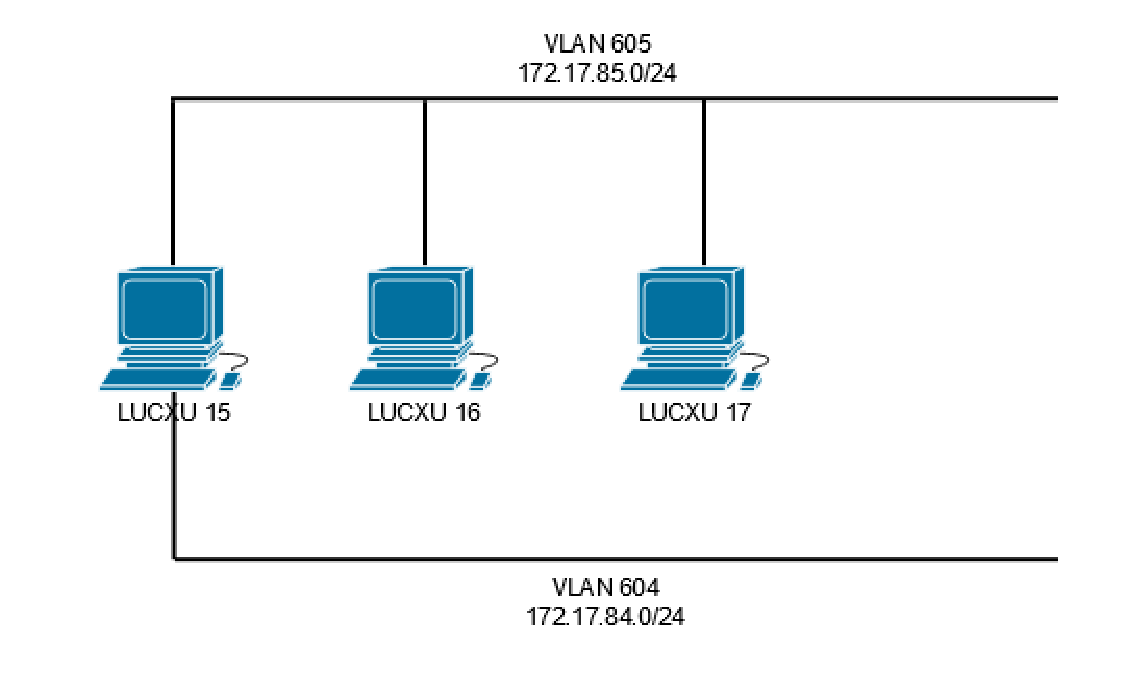
\includegraphics[width=\linewidth]{figures/network_schema}
  \caption{Network schema}
  \label{fig:network_schem}
  \end{center}
\end{figure}
For an easy use, The LUCXU15 workstation had two IPs address on the VLAN 604. On the VLAN 605, all the workstation have one IP address. The workstation LUCXU15 is working as a NAT router forwarding the traffic coming on VLAN 604 to LUCXU16 and LUCXU17.

\section{Documentation}
During the \gls{UAT} process, one important thing is to keep a trace to everything that is made. In order to do this, confluence is used. Confluence is a wiki webserver used as a co working software. A trainee section was reserved for the project and each part of the project is documented on it.

For an easy reuse, a document presenting an installation was done with a lot of screen-shot and command lines. 
\section{Log Management}
One problem that is present is how bring clear, synthetic and understandable log to the SIEM. This was not that simple because according to the network environment as shown on figure \ref{fig:network_schem}. Indeed, relevant logs that was coming from LUCXU16 and LUCXU17 have as IP source LUCXU15 (because of natting).

For example, an example of a log is : 

<156>Aug 20 15:41:47 heralding heralding \{"timestamp": "2019-08-20 13:41:44.925163", "duration": 0, "session\_id": "9c56927d-97a0-4039-b796-e9401cd145cd", "source\_ip": "172.17.85.50", "source\_port": 49316, "destination\_ip": "172.17.85.51", "destination\_port": 443, "protocol": "https", "num\_auth\_attempts": 1, "auth\_attempts" : [\{"timestamp": "2019-08-20 13:41:44.925968", "username": "nasty\_user", "password": "nasty\_password"\}], "session\_ended": true, "auxiliary\_data": \{"Host": "172.17.84.10", "User-Agent": "Mozilla/5.0 (Windows NT 10.0; Win64; x64; rv:60.0) Gecko/20100101 Firefox/60.0", "Accept": "text/html, application/xhtml+xml,application/xml;q=0.9,*/*;q=0.8", "Accept-Language": "fr, en-US ;q=0.7,en; q=0.3", "Accept-Encoding": "gzip, deflate, br", "Connection": "keep-alive", "Upgrade-Insecure-Requests": "1", "Authorization": "Basic YTph"\}\}

This is quite a long log but this is quite easy to parse so it is not such a problem. The context of this log is, for a testing purpose, I tried (IP address 192.168.180.117) to  join the server web on the IP address 172.17.84.10 with the credential nasty\_user:nasty\_password. The LUXCU15 workstation NAT the address to the honeypot server hosted on the LUXCU16 workstation. But the problem is here, if a SOC analyst sees this log, he will understand that someone is trying to connect to the honeypot but will not be able to investigate because the source IP address is the one of the LUCXU15 workstation (the nat router).\\
This is why what was done to make this problem not that important was to also generate nat log on the LUCXU15 workstation. Fortunately, iptables that is used to NAT allow some log. Here as the log in question:

<4>Aug 20 15:41:34 forwarder kernel: [4056859.198406] New Connection IN=eth1 OUT=eth0  MAC=00:50:56:be:3b:2a:00:1b:17:00:01:11:08:00 SRC=192.168.180.117 DST=172.17.84.10 LEN=52 TOS = 0x00 PREC=0x00 TTL=126 ID=51039 DF PROTO=TCP SPT=49314 DPT=443 WINDOW=64240 RES=0x00 SYN URGP=0 

We can see that there are the IP origin and the IP destination here. The correlation of the two previous log are now good for an analyst to investigate.

\section{Accepting Test}
For approving the solution, several tests are done. Two of them are presented here.
The first test that seems to be relevant was the most obvious one.
Let's begging with Nmap scanning. Nmap is a free open-source software used to identify open ports, operating systems and get information about services running on a specified address IP.
We can see below the response of nmap scanning on the two exposed IP on the VLAN 604.

Nmap scan report for lucxu15.int.excellium.lu (172.17.84.10)\\
Host is up (0.015s latency).\\
Not shown: 984 closed ports\\
PORT     STATE SERVICE\\
21/tcp   open  ftp\\
22/tcp   open  ssh\\
23/tcp   open  telnet\\
25/tcp   open  smtp\\
80/tcp   open  http\\
110/tcp  open  pop3\\
143/tcp  open  imap\\
443/tcp  open  https\\
514/tcp  open  shell\\
993/tcp  open  imaps\\
995/tcp  open  pop3s\\
1080/tcp open  socks\\
3306/tcp open  mysql\\
5432/tcp open  postgresql\\
5900/tcp open  vnc\\
9000/tcp open  cslistener\\

This is working, all services are on one single port but in production, there will be on several IPs addresses. Looking to Qradar after this is showing a lot of alert showing that the system was scanned.

The Canary tokens also have to be tested. For an easy test, a docx file was created with the name secret\_password.docx. After having successfully created this document. The file was dropped on the Windows Share. When someone opened the file, this log was send to the SIEM :

<164>Aug 20 15:32:26 heralding webhook {"additional\_data":{"location":null,"referer" : null,"src\_ip" : "192.168.180.117","useragent": "Mozilla/4.0 (compatible; MSIE 7.0; Windows NT 10.0; Win64; x64; Trident/7.0; .NET4.0C; .NET4.0E; .NET CLR 2.0.50727; .NET CLR 3.0.30729; .NET CLR 3.5.30729; ms-office; MSOffice 16)"},"channel": "HTTP", "manage\_url" : "http://172.17.84.10/manage?token=[...] auth=62f02306e397af03283b66a606c23a7a" ,"memo":"Test Meeting Mathieu","time":"2019-08-20 13:32:18"}

This is a very good log because in one log an investigation could be made. The IP address of the computer that triggered the document is here, there is also the remember message and the link of the server where there is more document available. 
 

\cleardoublepage
\chapter{Client deployment}
\section{Preparation}
Before coming into the client, a preparation sheet should be written. In the following of UAT implementation, two documents have been written. The first one is a document dealing with the installation process and the second one is a document that needs to be filled by a client network administrator.\\
The first document is written with the help of all the note taken during the UAT development. It defines all the processes that need to be done. First this is how to set up an installation from a template, then this is what script or command to run with what argument.\\
The second document is sent to the client. This is a document that is sent in order to gather private information that will be needed for the deception system installation. The list of information ask is: 
\begin{itemize}
    \item DNS IPs,
    \item Fixe IP address,  
    \item Vlans accessible,
    \item Email of the supervisor,
    \item Phone number of supervisor.
\end{itemize}


\section{Deployment}
Unfortunately, at a time where the memory is written, the deployment is not yet finished.


\cleardoublepage


\chapter{Review of the Project}
This was a project that last six months. After a time like this, it is mandatory to do a recap of what was done, was could have been better and what was good. It is also important to see where the project goes and what are its impacts.

\section{Axes of improvement}
Unavailable, after six months errors occur and lessons have to be taken. \\
The first thing that could have been improved is my research process. I think that I should have maybe spent less time at the beginning, do some design and then do again some research. This could have help me to face some technical issues. I also think that I should have been more precise during the creation of the Gantt because during the middle of the internship, I lost myself doing some research. This could be avoided if every task as a beginning and an ending phase. 

\section{Project becoming}
The project deliverable is available via confluence access to the trainee folder. The project, after what I've done will be taken by the members of the CSIRT. There will aslso have some training sessions to SOC enginieers and analysts for explaining to them what is the project about and to what correspond the alerts.


\section{\gls{Excellium} Impact}
This part will be dealing about the impacts that the project had on Excellium and the CSIRT.
Firstly, the project allows Excellium-services to beef up their portfolio of services that they can provide. That means that if some client of Excellium heard about deception or honeypot technologie, Excellium can provide them my project.
One other impact is that the global knowledge of Excellium is growing. Indeed, the work I did about state of the art and the deployment is steal here and can help for other projects. The POC that I did will be a good start for anything looking like that.


\cleardoublepage


\chapter{Project Management}
\blt{T}{he} project assigned to me was a complete one. I needed first to understand what was the technologies already in place, what design I wanted for the project, I also needed to implement a test of this solution in \gls{Excellium} \gls{UAT} and finally I had to implement it in a client infrastructure.

With this in mind, several parts of the projects (see picture \ref{fig:Gantt}) came up: 
\begin{itemize}
    \item State of the Art: the part of gathering information,
    \item Design: the part of designing the solution,
    \item Deployment \gls{UAT}: the part of the first deployment and testing the solution,
    \item Deployment Production: the part where the solution is test on a client infrastructure.
\end{itemize}
With this in mind, and some discussions with my industrial supervisor, we came up with a previsional Gantt which is shown on the top of the figure \ref{fig:Gantt}. The beginning of the project was perfectly respected. The Deployment on the \gls{UAT} of \gls{Excellium} took more time that expected because of some trouble that I had technically speaking and also because I had a car accident that put me in labor disruption. As a result, as it is shown in figure \ref{fig:Gantt}, three more weeks was spent on the \gls{UAT} deployment.


\begin{figure}[h!]
  \begin{center}
  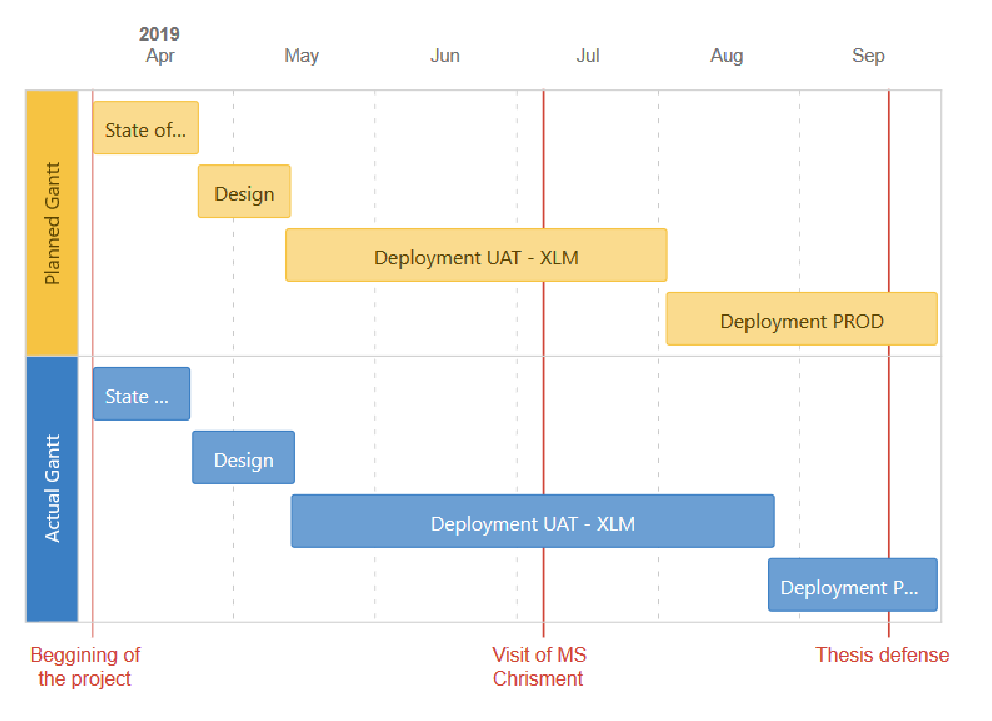
\includegraphics[width=\linewidth]{figures/Gantt2}
  \caption{Previsional Gantt vs actual}
  \label{fig:Gantt}
  \end{center}
\end{figure}


Some other tasks was obviously present during the project and planned on the Gantt but they are not shown in the figure \ref{fig:Gantt} with a view to making things clearer. There are the detail presentation of these tasks not mentioned on the Gantt: 
\begin{itemize}
    \item Project Management: to have a better view of the project, the plan was to have a weekly review on the Friday with my industrial manager. Those weekly review have two main goal, the first is to see if the project is going well and if we have to change something in the Gantt. The second goal is to see if I have any question and giving me path of reflections.
    \item Reporting: a part of my working hours was dedicated to the writing of my master thesis. Four hours was dedicated to the writing of my report every week.
    \item Documentation: this task goes in pair with the previous one. When the previous was for academical purpose, this one was for industrial purpose. Indeed, knowing the fact that the project will maybe be taken by someone else after my internship, all that I did need to be documented for a quick understanding. The time allowed to this was share with the reporting one because, a lot of time, what was put on my documentation section was also in my report, and vis versa.
    \item Training: Some time, some training was given in the company and I had the chance to attend them. The time dedicated to this was very punctual, I spent twenty hours at the most.
    \item CERT XML duty: As explained in the section \ref{certxml}, I had the chance to see and do some actual daily \gls{CSIRT}'s job. The time spent for each activity was very variant. The news lasts one hour when the Newsletter lasts one complete day.
\end{itemize}






\cleardoublepage


\chapter{Conclusion}
The project objective was to build a deception system from A to Z. I first learn a lot about deception technology as an all and wrote a state of it. Then, I had to think about how doing it and how to present it. After, I built a first version of what I designed and test it. Finally, I tried it on a client environment. We could say that the objective that was fixed in the begging was followed. 

I learned a lot during this project regarding many topics. Of course about cybersecurity but also about networking that is a mandatory topic in computer science. I also learned how to lead a project from its begging to a production and all the project management that is behind. This is also a great feeling to apply what I study during my years in Telecom Nancy. I could see that something that I thought meaningless could be very important and also what I thought important could not be. But most importantly I think that this internship was a human journey. It makes a bridge between student life and the adult working life that I will certainly have for the forty next year of my life. 

The project strengthens my wish of working in the cybersecurity area and helping build a safer numeric  world. 



\cleardoublepage
\renewcommand{\tocbibname}{Bibliographie / Webographie}
\bibliography{biblio.bib} % See example.bib
\bibliographystyle{plain}

\cleardoublepage

\listoffigures
\cleardoublepage

\listoftables
\cleardoublepage

%\lstlistoflistings
%\cleardoublepage

\printglossaries

\cleardoublepage
\renewcommand{\thesubsection}{\Roman{subsection}}

\appendix
%\part*{Appendix}
%\addcontentsline{toc}{part}{Appendix}
%\cleardoublepage

%\chapter{First Appendix}
%\cleardoublepage

%\chapter{Second Appendix}

%\cleardoublepage
\thispagestyle{empty}

\section*{Résumé}
\addcontentsline{toc}{chapter}{Résumé}

Ce mémoire d'ingénieur décrit le projet que j'ai mené lors de mon stage de fin d'étude dans l'entreprise Excellium au Luxembourg. Lors de ce stage, j'ai été amener à élaborer et à mettre en place un système de deception. La deception est un concept qui reprend le concept plus connu des 'honeypots' ou pots de miels qui ont pour principe de leurrer un potentiel attaquant en imitant un faux serveur. Le principe de deception est un peu plus étendu que celui des pots des miels et ne se limite pas qu'à la création de faux serveurs. La solution que j'ai élaborée est détaillé et chaque choix effectué est justifié. Une partie de gestion de projet et un bilan du projet sont également disponible.

{\bf Mots-clés:} Deception, Honeypot


\section*{Abstract}
\addcontentsline{toc}{chapter}{Abstract}

This master thesis describ the project that I realized during my final intership in the company Excellium in Luxembourg. During this internship, I was led to develop and set up a deception system. Deception is a concept that takes up the well-known concept of honeypot which principle is tricking a potential attacker mimicking a fake server. The principle of deception is a little more extensive than that of honeypots because is not limited to the creation of fake servers. The solution I developed is detailed and each choice made is justified. Project management and a review of project are also available.



{\bf Keywords:} Deception, Honeypot 

\end{document}
